% !TeX spellcheck = en_US

\section{Filter Comparison}

\subsection{Architectural differences}
The main difference of each pack of filters is the architecture itself.
Using a standard multiplier, the filter coefficients are multiplied with the input samples using multipliers. The output is obtained by summing the products of the coefficients and input samples. This architecture is straightforward and produces accurate results but can be resource-intensive in terms of hardware implementation.

The second implementation is by using factored CSD., This is a technique used to reduce the number of partial products required for multiplication by decomposing the coefficients into a sum of powers of two. This architecture employs a combination of shifters and adders to implement the multiplication operation. The output is obtained by accumulating the partial products. Factored CSD reduces hardware complexity and power consumption compared to the multiplier architecture, but it may introduce some additional round-off errors due to approximation.

The last architecture used in this project is called Distributed Arithmetic (\emph{DA}).
Distributed arithmetic is another technique for efficient multiplication using look-up tables (LUTs). In this architecture, the filter coefficients are precomputed and stored in a LUT. The input samples are used as indices to retrieve the corresponding precomputed values from the LUT. These values are then summed to obtain the filter output. Distributed arithmetic offers advantages in terms of reduced hardware complexity and power consumption but can introduce quantization errors due to the finite precision of the LUT.

So, when comparing these architectures, we can expect the multiplier architecture to provide the most accurate results but at the cost of increased hardware complexity and power consumption.
The factored CSD and distributed arithmetic architectures offer trade-offs by reducing hardware requirements and power consumption while introducing minor approximations that result in slight differences in the output.

\subsection{Minimum Order filter}
Beginning with the minimum order one using floating point precision (\textit{32 bits}), we can observe that the created circuit can barely fit inside the target FPGA. As we can see from the figure~\ref{fig:fir_min_dsp_util}, DSP utilization is at $100\%$ and drops almost linearly with the decrease of bits used in computation. Note that, DSP utilization is $0\%$ when using 8 bits arithmetic because of the compiler being able to do every computation needed using LUTs and flip-flops.

The same pattern can be observed in the 2-stage multiplier architecture as the number of computations didn't decrease. Increasing pipeline stages from one to two, theoretically, increases operations per cycle but it didn't have the same impact on execution time. From table~\ref{table:multiplier_stages_time}, we can see that execution time of 1-stage pipeline is faster than 2-stage pipeline by $20\hspace{3pt}ns$. This decrease in execution time is due to several overheads from the second pipeline stage but the increase of those stages can increase efficiency by dropping operating frequency while doing the same amount of computations in the same time (\textit{because of the reduced slack}).

\begin{figure}[htbp]
	\centering
	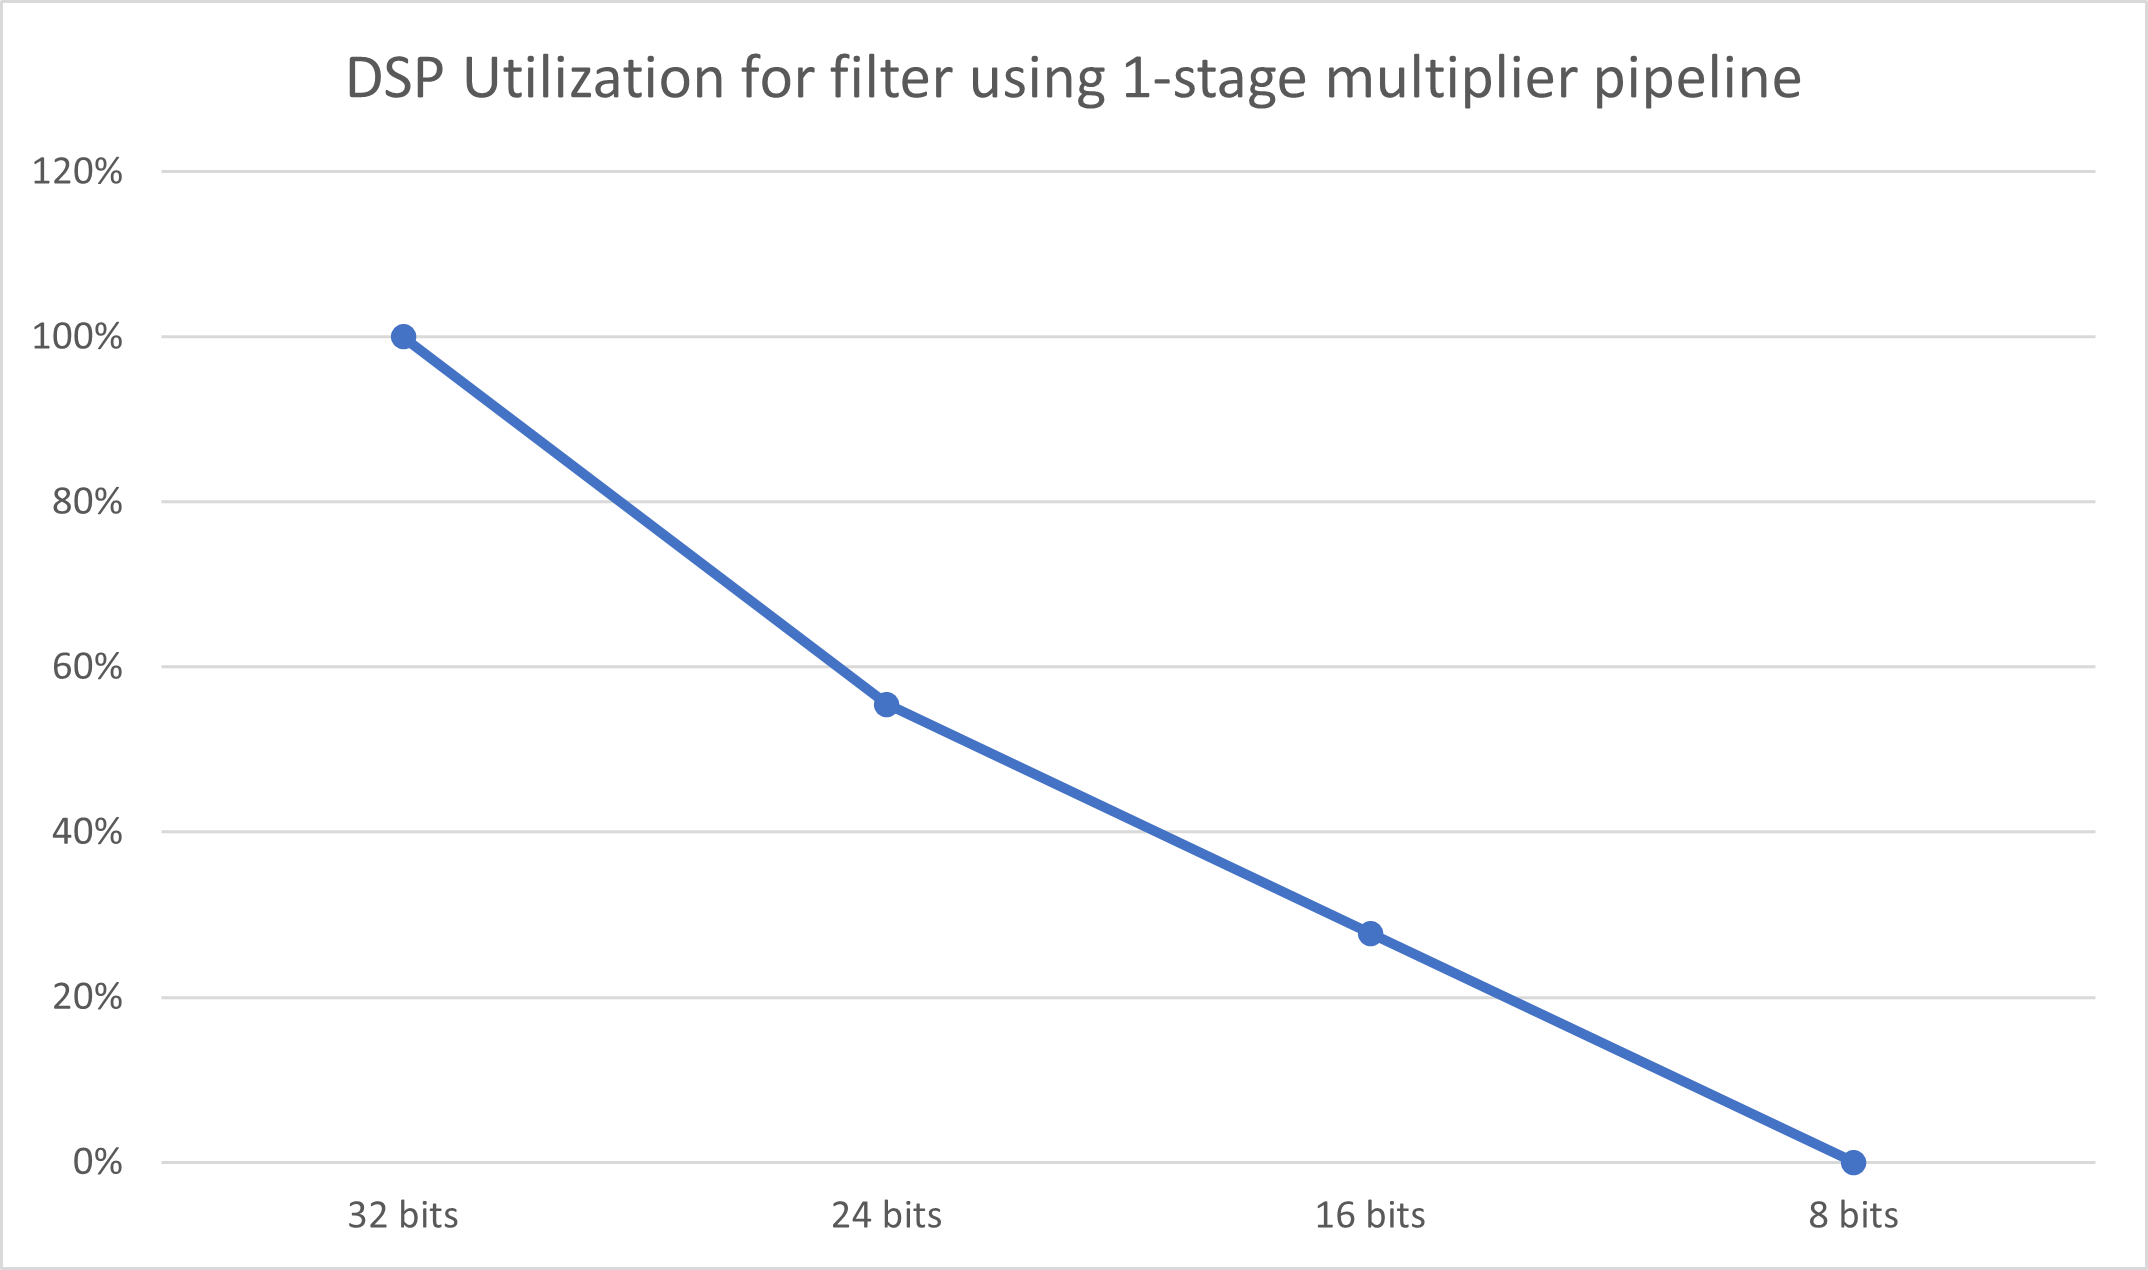
\includegraphics[width=0.45\textwidth]{../Images/FIR_min_Order/multiplier_1_pipeline/dsp_util.png}
	\caption{DSP utilization for min. order filter (\textit{multiplier 1-stage}) using different bits}
	\label{fig:fir_min_dsp_util}
\end{figure}

\begin{table}[htbp]
\centering
\begin{tblr}{|c|c|}
	\hline
	Architecture & Time \\
	\hline
	{Multiplier 1-stage pipeline} & 35140 ns\\
	\hline
	{Multiplier 2-stage pipeline} & 35160 ns\\
	\hline
\end{tblr}
\caption{Time for different multiplier pipeline stages using 32 bit floating point arithmetic.}
\label{table:multiplier_stages_time}
\end{table}

Knowing the latency of each architecture, we can calculate the overall execution time for a specific sample set. MATLAB's sample set consists of $3499$ samples. So, using the following formula, we can calculate each architecture's execution time.
\begin{small}
\begin{equation}
	\centering
	\begin{split}
		Execution\hspace{3pt} time &= \\
		& \hspace{-55pt} =\frac{{Latency \hspace{3pt} per \hspace{3pt} sample}\cdot{Number \hspace{3pt} of \hspace{3pt} Samples}}{{Clock \hspace{3pt} frequency}}
	\end{split}
\end{equation}
\end{small}
By inserting numbers in the formula above, we get the diagram that is displayed in fig~\ref{fig:exet_time_min_32b}. Clearly, execution time follows the gradient of latency per sample.
Moving on to the multiplier-less factored CSD architecture, we can start to observe a significant decrease in latency per sample, at first, and then in execution time, as this architecture outputs a new value at least 2 time-units quicker than any multiplier architecture mentioned above. This architecture achieves this speed by using small approximations on the output, which increase overall speed but does not affect much the filter's output.

%\begin{figure}[htpb]
%	\centering
%	\subfigure[HDL latency for different architectures in samples.]{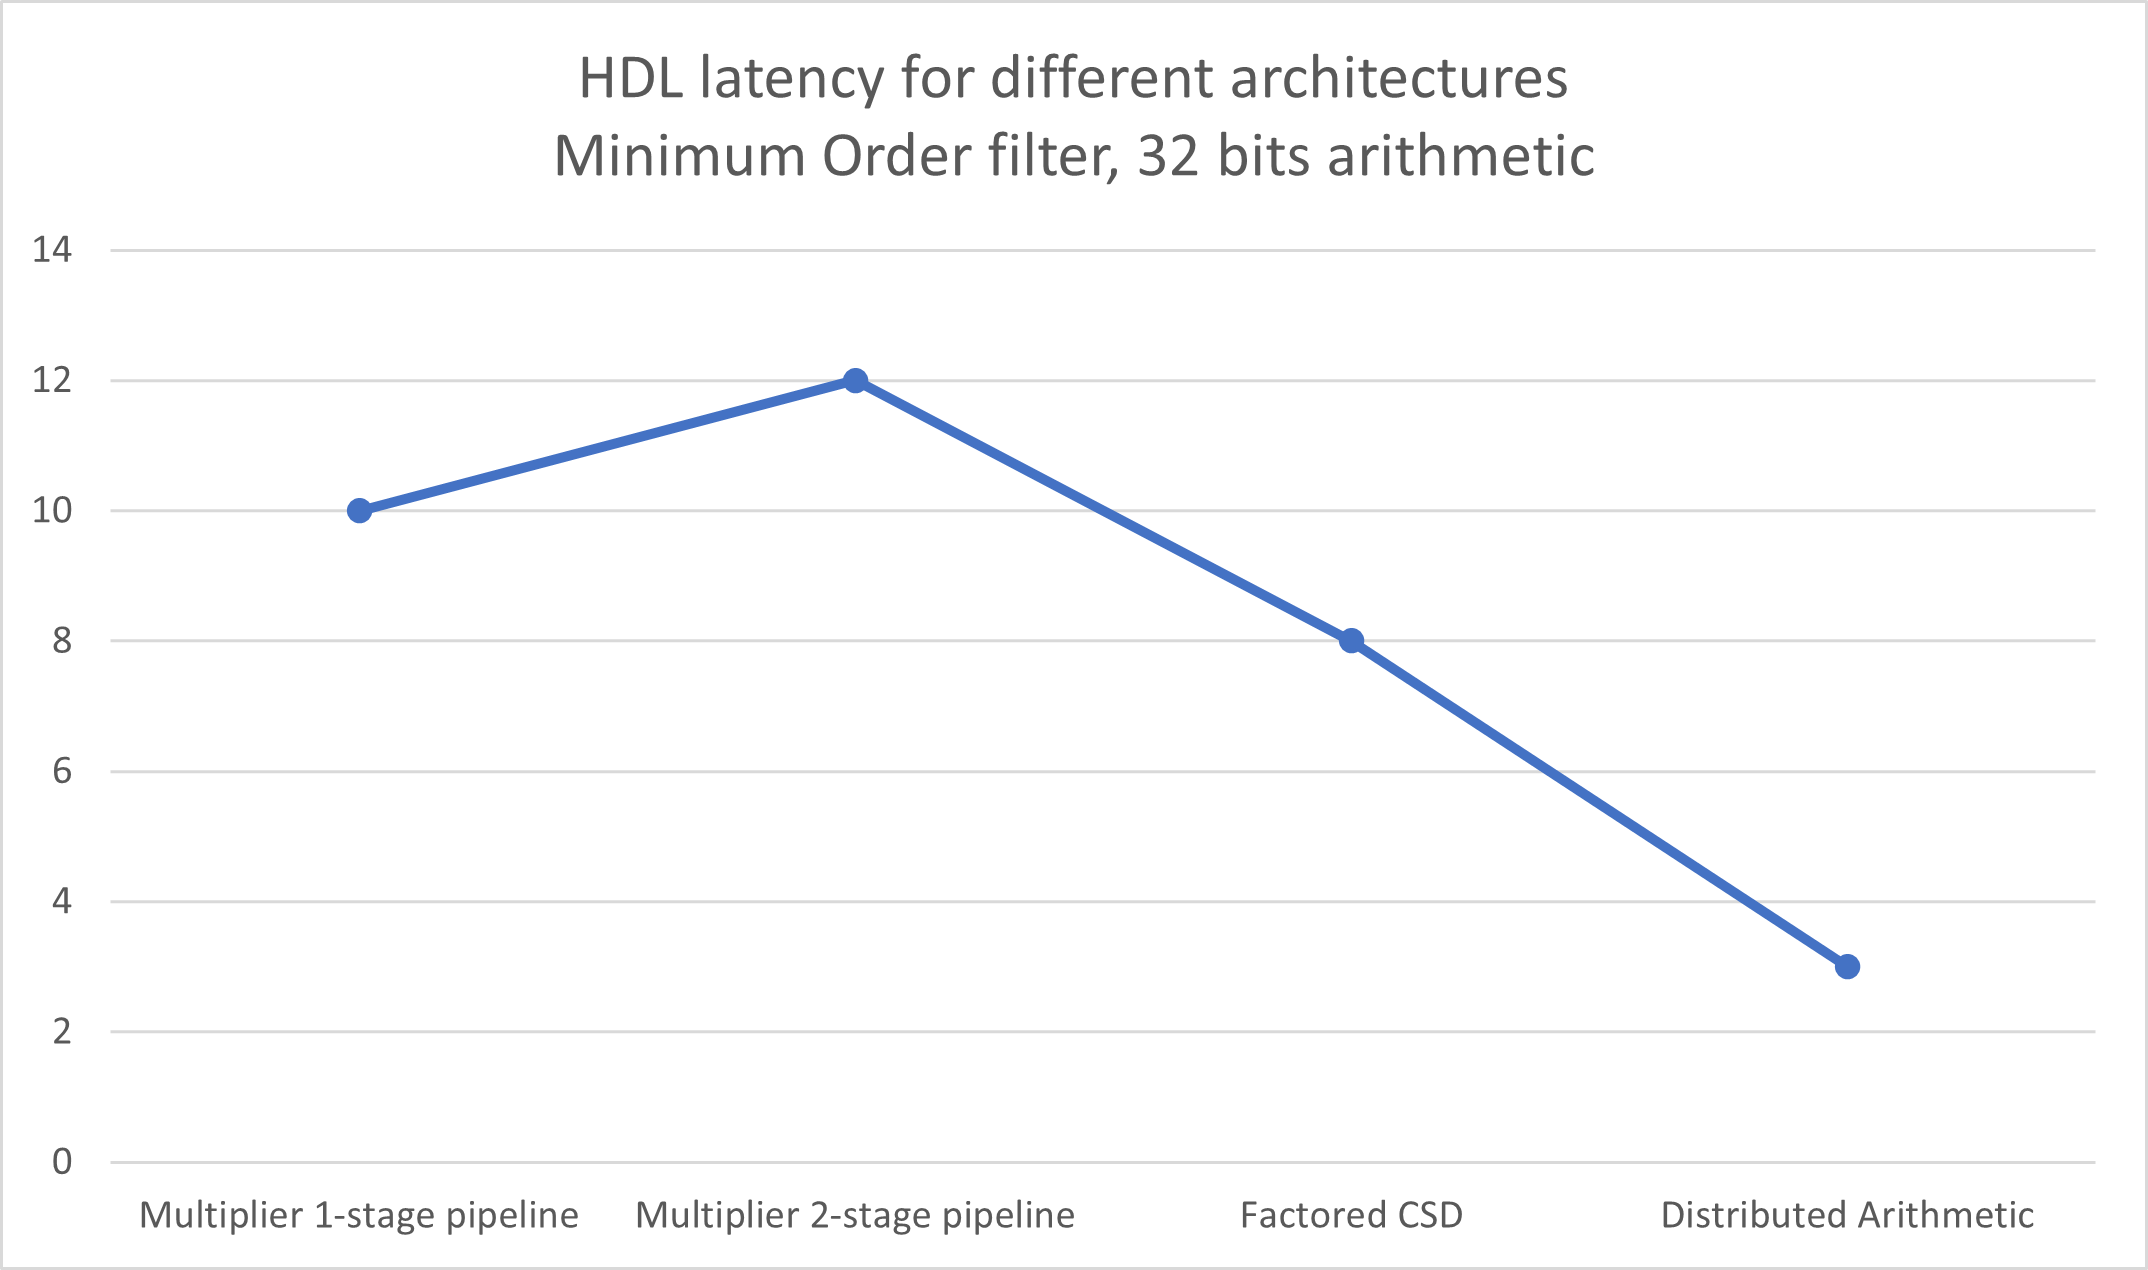
\includegraphics[width=0.45\textwidth]{../Images/FIR_min_Order/hdl_latency_32bits.png}}\\
%	\subfigure[Execution time for different architectures in seconds.]{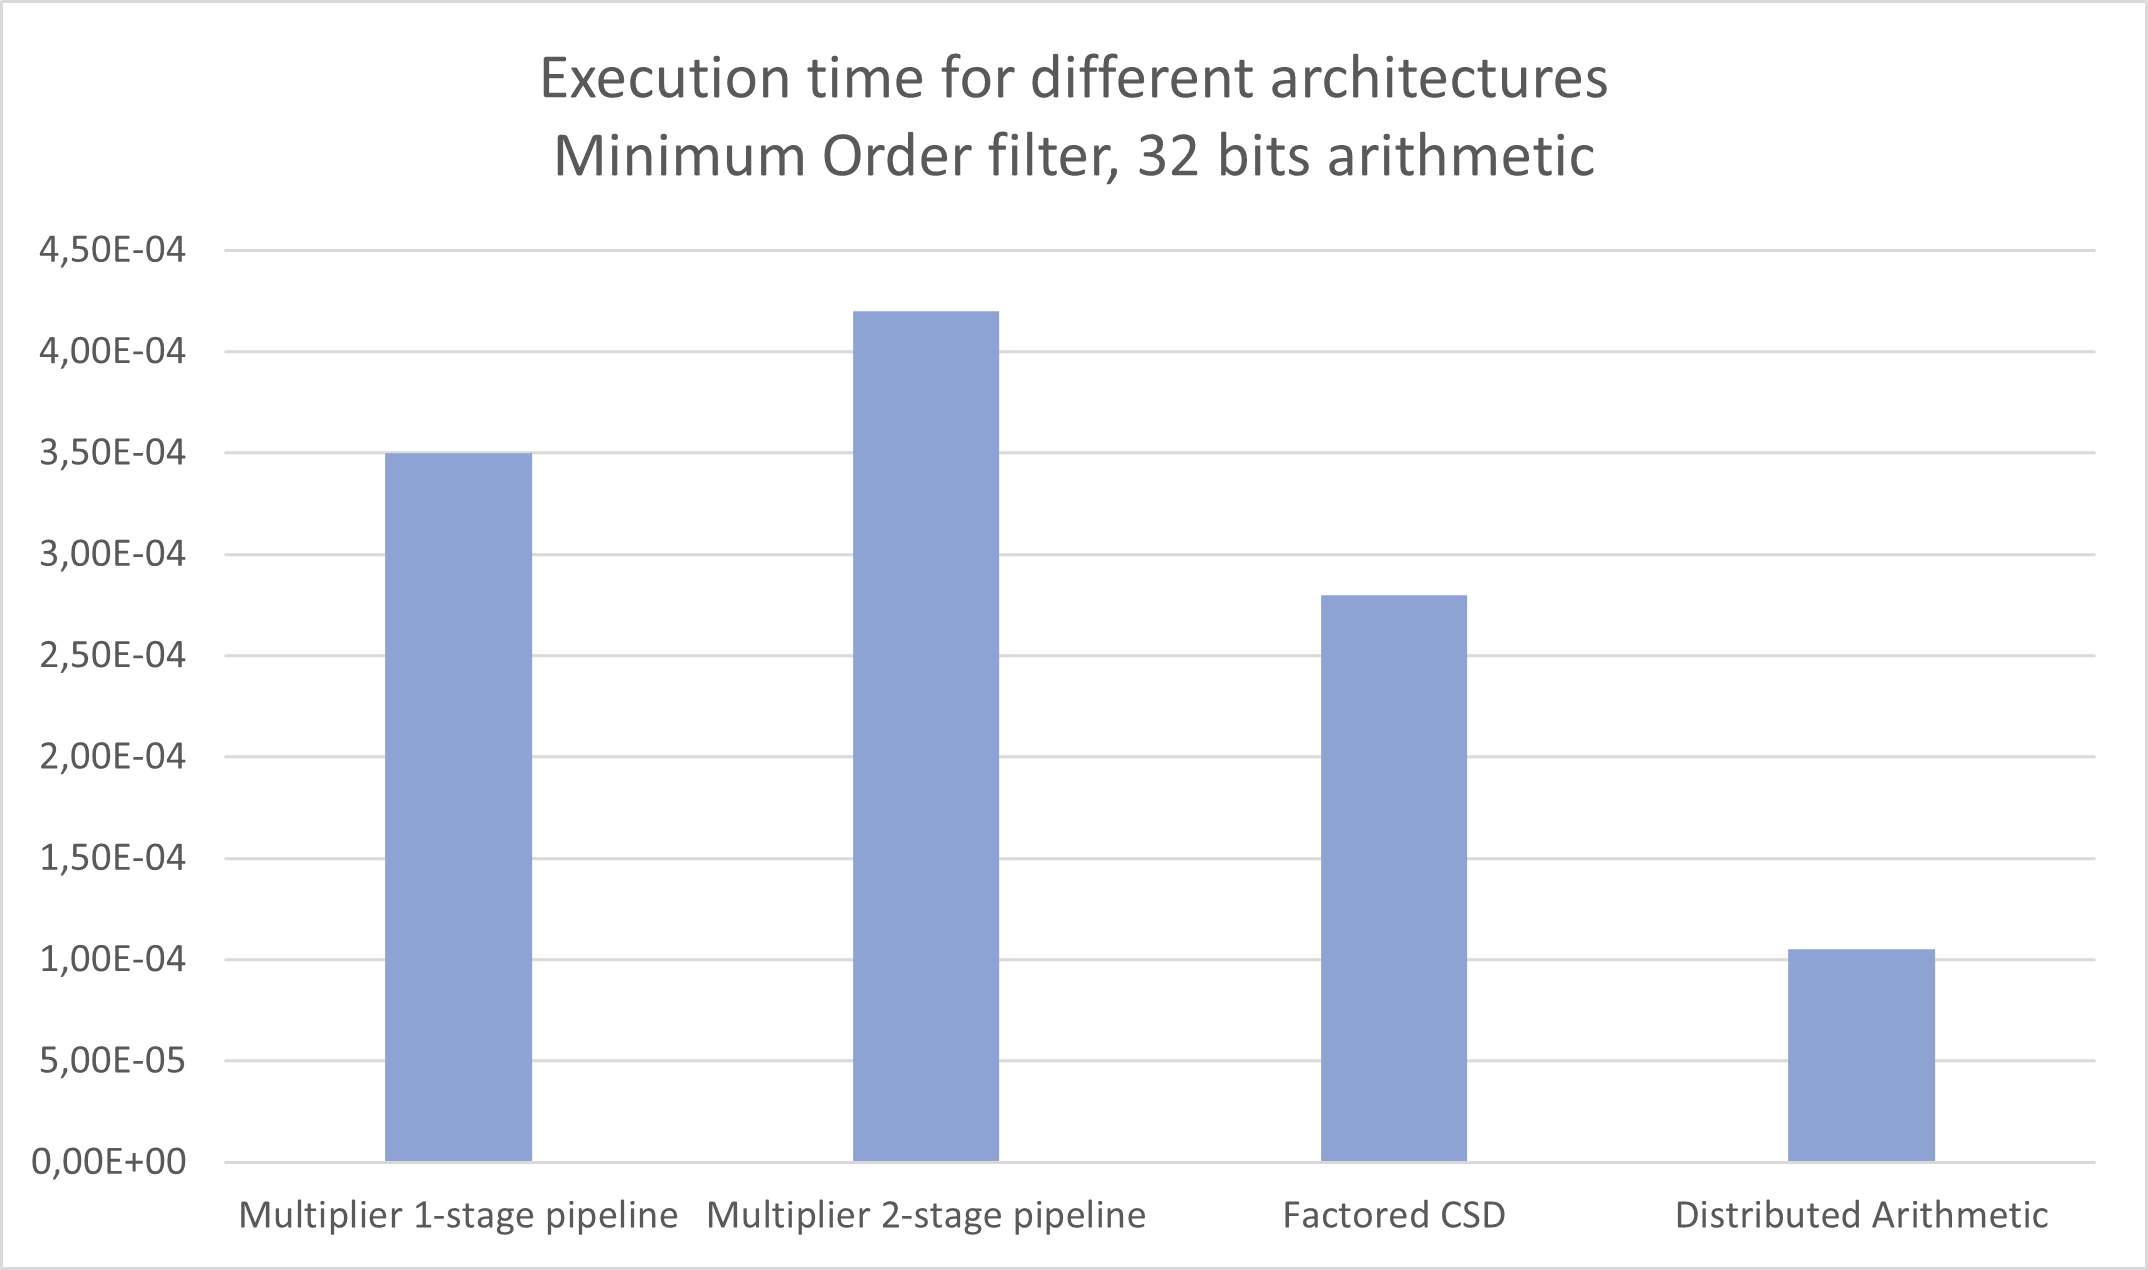
\includegraphics[width=0.45\textwidth]{../Images/FIR_min_Order/exec_time_32bits.png}}
%	\caption{Latency and execution time for different architectures.\\ \textit{Note: This is for 32bit arithmetic, the same pattern is observed for the other arithmetics.}}
%	\label{fig:exec_time_latency_min_32}
%\end{figure}

\begin{figure}[htbp]
	\centering
	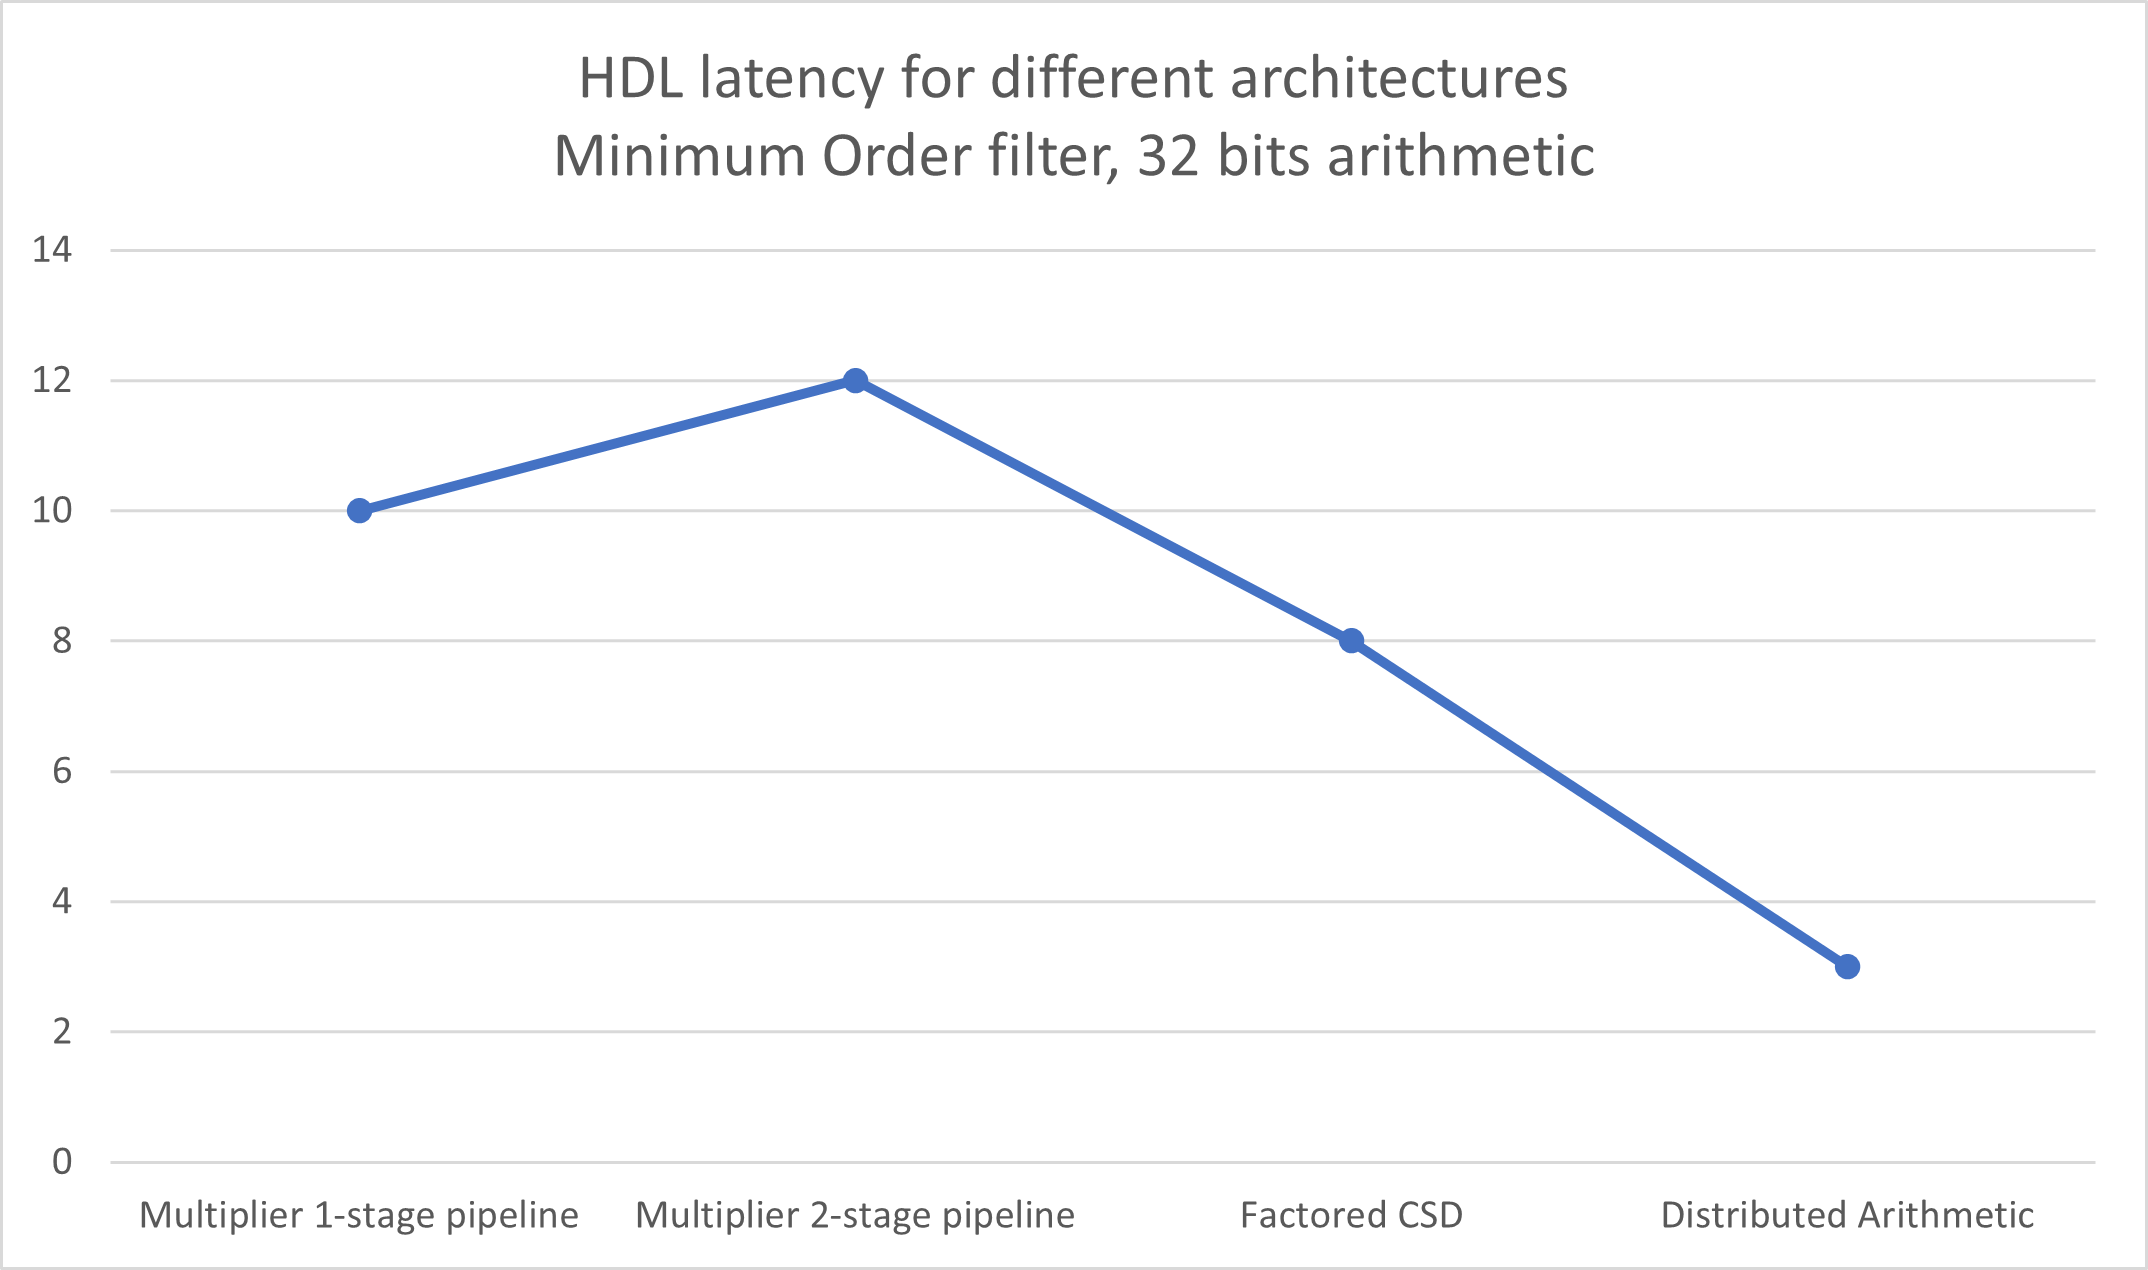
\includegraphics[width=0.45\textwidth]{../Images/FIR_min_Order/hdl_latency_32bits.png}
	\caption{HDL latency for different architectures in samples.\\ \textit{Note: This is for 32bit arithmetic, the same pattern is observed for the other arithmetics.}}
	\label{fig:hdl_latency_min_32b}
\end{figure}

\begin{figure}[htpb]
	\centering
	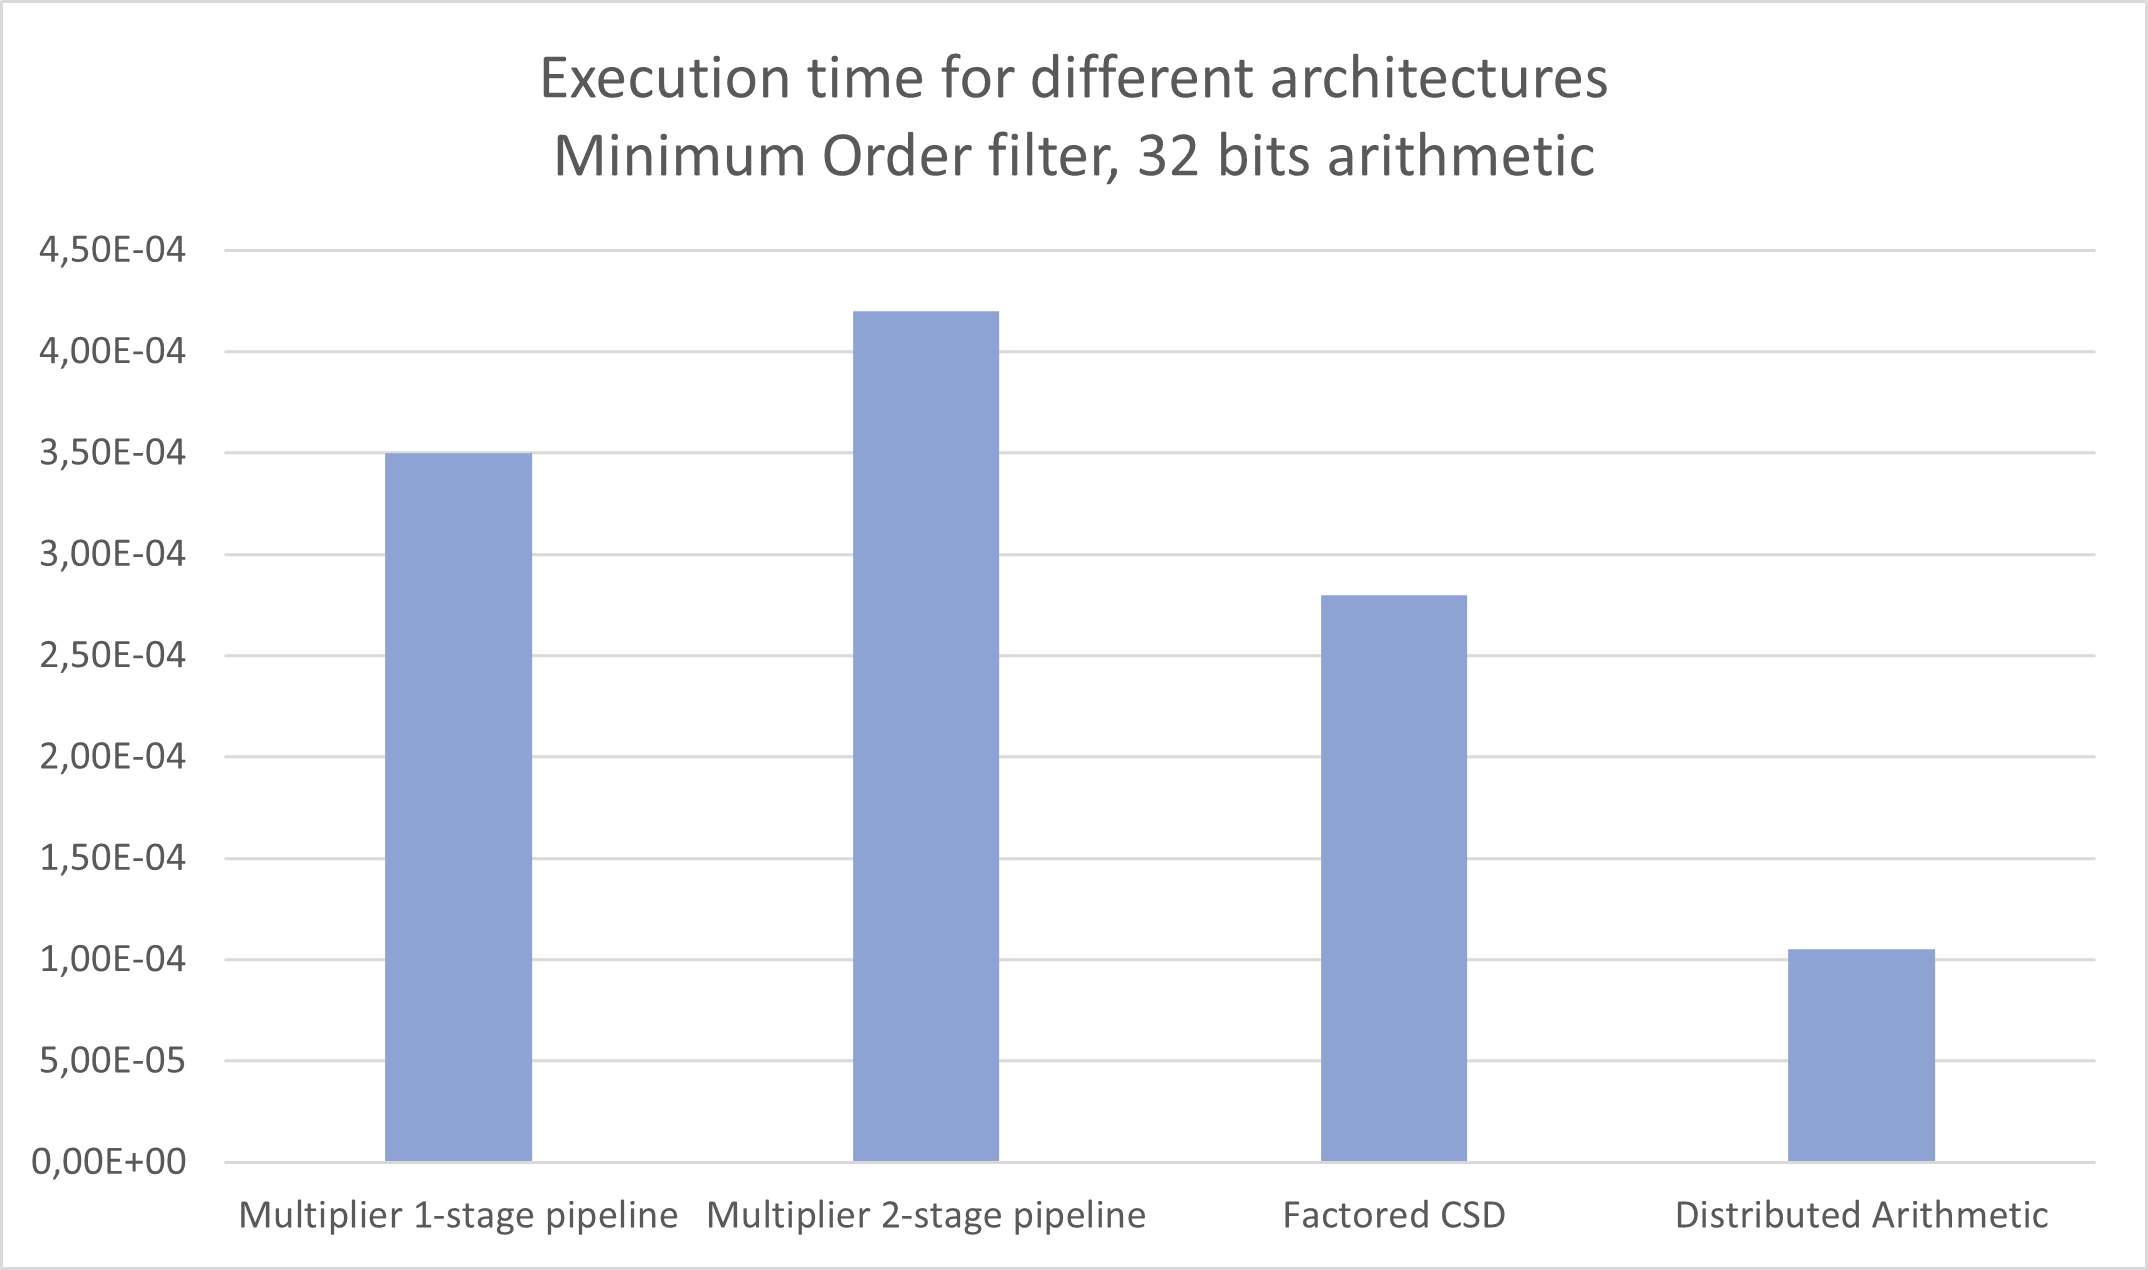
\includegraphics[width=0.45\textwidth]{../Images/FIR_min_Order/exec_time_32bits.png}
	\caption{Execution time for different architectures in seconds.}
	\label{fig:exet_time_min_32b}
\end{figure}

Finally, the distributed arithmetic architecture seems to be the most quick of all above architectures as viewed in figure~\ref{}. Also, this architecture appears to be the most efficient of all since no DSP block is used and LUT utilization is smaller than that of other architectures. However, this comes to a cost which is using approximations as "normal" output. Those approximations produce results that have been approximated more than those produced by the factored CSD architecture.

\subsection{20 Order filter}

\subsection{30 Order filter}
